\section{\ref{algo:htf} Algorithm}

One of the main drawbacks of the \simpleAlgo and \multipleAlgo Algorithm is the lack of a retracting mechanism. That is, once a flowset did not have enough frequency and was split further, we will not reconsider it again. The \ref{algo:htf} Algorithm remedies the lack of this mechanism.

We note that at the first round, the previous algorithms partition the space of flows into disjoint flowsets depending on the number of counters. At this initial step, all possible flows are covered by a single flowset. However, once a splitting decision is taken, only suspect flowsets will be partitioned and other flowset will stop being monitored. This  usually keeps a vast part of the flow space uncovered.

In order to overcome this, the \ref{algo:htf} Algorithm tries to retract up the hierarchy the part of the flowsets that previously were not be monitored. This retraction will come at a cost of not freeing those counters to measure more refined flowsets as before. Thus, the retraction should be to the highest level possible in the hierarchy.

When considering up to which point to retract these flowsets, one should consider two main aspects. The first one is retracting to the highest level while still not having a flowsets which is above the threshold.  Such flowsets are likely to split once again at the next round. The other consideration is to monitor flowsets which consist a frontier of the whole flow space and still maintain a disjoint partition.

\begin{figure}
	\centering
    \subfloat[First Round Frontier]{
        \label{subfig:first_round}{
        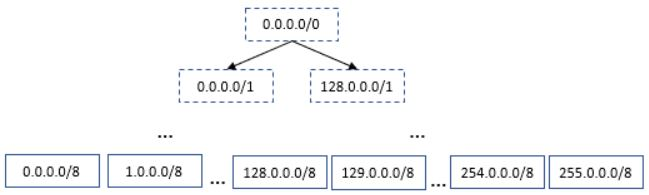
\includegraphics[width=\linewidth]{HHH/jpg_figures/retract1.JPG}
        }
    }
    \hfill
    \subfloat[Second Round Frontier] {
        \label{subfig:second_round}{
        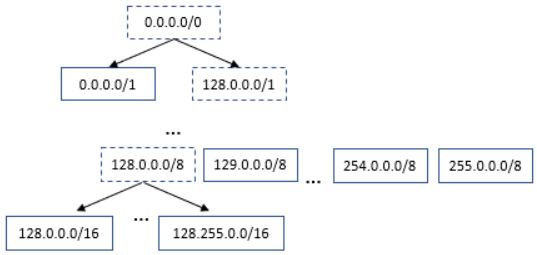
\includegraphics[width=\linewidth]{HHH/jpg_figures/retract2.JPG}
        }
    }
\caption{An example of the retraction mechanism in \ref{algo:htf} Algorithm.}
\label{fig:retract}

\end{figure}

Figure~\ref{fig:retract} depicts an example of the retraction mechanism in action for an IP\_SRC hierarchy. In this figure, the CIDR mask inside the nodes represents the flowset of this node. Furthermore, nodes with full outline are the monitored nodes, while nodes with dashed outline are non monitored nodes.

At the first round, the algorithm starts monitoring the whole flow space at level 8. As a result of the monitoring in the first round, the algorithm decided to split only the flowset $128.0.0.0/8$ because it is the only flowset that surpassed the threshold. Instead of simply abandoning the other flowsets, the algorithm tries to recursively retract to the highest level.

This recursive retracting start by classifying all flowsets at the current level into several categories: refine, keep and retract. flowsets that are classified as refine are flowsets that surpasses the threshold, these flowsets are interesting and the algorithm  partitions them in a lower level at the next round. Flowsets that are siblings of refine flowsets will be classified as keep, these flowsets did not surpass the threshold but can not be retracted to higher level since their siblings are refined. All other flowsets are classified as retract, and are aggregated into their common ancestor at a higher level.

We note that once  two siblings are classified as retract at level $l$, then their common ancestor is added at level $l-1$. When processing the level $l-1$, if this ancestor surpassed the threshold then these two siblings will be added back to the frontier at level $l$ as refine of level $l-1$.

However, when the algorithm decides on the refine set at the currently monitored level, it might partition these flowsets more than one level down the hierarchy as the case with the \multipleAlgo Algorithm, depending on the configurations.

Subfigure~\ref{subfig:second_round} depicts the frontier after the retraction process. The flowset $128.0.0.$- $0/8$ was in the refine set of level 8 and thus was refined into the flowsets $128.0.0.0/16$ up to $128.255.0.0/16$. The flowset $129.0.0.0/8$ was classified as a keep in level 8 since its sibling was classified as a refine in the same level. The flowsets in the range of $0.0.0.0/8$-$127.0.0.0/8$ were not active during the first round, and thus were retracted up to level 1 and will be monitored by a single counter at the flowset $0.0.0.0/1$. The flowset $0.0.0.0/1$ was classified as keep at level 1 since its sibling was not present when level 1 was process, meaning it was partitioned at lower levels.

The flowsets $254.0.0.0/8, 255.0.0.0/8$ did not surpass the threshold thus were not classified as refine at level 8 and thus should be retracted, but assuming that their common ancestor $254.0.0.0/7$ did surpass the threshold and were classified as refine, they were added back to the frontier at level 8.

Up to this point we overlooked and important detail of the retracting mechanism, the affect of retracting on the number of available counters. In the best case scenario, the retracting mechanism manages to retract vast parts of the frontier to higher levels and saving enough counters, more than needed for refining flowsets at the refine set of the current level. In this scenario, the algorithm still managed to keep the frontier intact, covering the whole space, and to refine the interesting flowsets as needed.
If additional counters are available, the algorithm unretracts higher levels by refining their flowsets.

This unretacting step, happens only if we saved enough counters, and the motivation behind is to set the algorithm in better position for the next round. That is, since we have spare counters after all the required refinements, we partition flowsets at the higher position of the hierarchy into a lower level since these flowsets are the most aggregated and are the most prone to surpass the threshold without any actual child that surpasses the threshold.

On the other hand, in the worst scenario the retracting mechanism does not save enough counters to enable full refinement of the frontier. This scenario might happen in a balanced trace over the hierarchy where the algorithm does not manages to retract the frontier up to the higher levels. While the most common possibility of this scenario is that the number of counters is in the order of the number of HHH in the trace. In such scenario, the algorithm does not have enough counter for full refinement and for keeping the frontier intact since the set of suspect HH are in the order of the number of the available counters and the algorithm track each suspect HH by a single counter at each point.

The complexity of the retracting and unretracting step of this algorithm is still $O(HC)$, since at most we perform recursive retraction over $(H)$ levels and unretracting over the same $O(H)$ levels. The most important thing to note when considering the complexity, is that at any given level we perform at most $O(C)$ operation and not $O(2^l)$ operations, since  at each level the algorithm monitors at most $O(C)$ flowsets and when performing the classification of each level we consider only monitored flowsets.

Thus, despite complicating the per round operation the algorithm still performs a constant per-packet operation and a constant number of times a  heavier operation that is still linear in the number of counters and $O(1)$ when considering the number of packets or even the number of active flows.
\begin{algorithm}\small
    \SetKwInOut{Input}{Input}
    \SetKwInOut{Output}{Output}
    \Input{A stream of packets $S$, a threshold $\phi$, number of counters $C$ and the depth of the hierarchy $H$}
    \Output{set of HH and HHH in $S$}
    $F = init\_flowsets(C)$\;
    $levels=calculate\_levels(C,H)$\;
    $current\_level=levels[0]$\;
    $number\_rounds=|levels|$\;
    \ForEach{$r$ in $\{1..number\_rounds\}$}
    {
        $counters=assign\_counters(F)$\;
        $P=get\_round\_packets(r, number\_of\_rounds)$\;
        \ForEach{$counter$ in $counters$}{
            counter.value=$\sum\limits_{\{p\in P : flow(p)\in counter.flowset\}}value(p)$\;
        }
        \If{$r < number\_rounds$}
        {
            $l=levels[r]-current\_level$\;
            $to\_refine, retracted = retract\_frontier(counters, F, current\_level)$\;
            $refined = refine\_flowsets(to\_refine,l)$\;
            $needed\_counters = |refined \cup retraced|$\;
            \If{$needed\_counters > C$}{
                $abort()$\;
            }
            \Else{
                $retracted = unretract\_frontier(C - needed\_counters, retracted)$\;
            }
            $F=refined \cup retracted$\;
        }
    }
    return $calculate\_hhh\_bottom\_up(\phi)$\; 
    \ignore{
    $hh\_per\_level=calculate\_hh\_per\_level(\phi)$\;
    $hhh\_per\_level=calculate\_hhh\_per\_level(\phi, hh\_per\_level)$\;
    return $hh\_per\_level, hhh\_per\_level$\;
    }
    \SetAlgoRefName{\htfAlgo}
    \caption{}
    \label{algo:htf}
    \vspace{-0.1cm}
\end{algorithm}
